\textcolor{blue}{Problem 5}

7.34 Capacity. Find the capacity of \\
(a) Two parallel BSCs: \\
(b) BSC and a single symbol: \\
(c) BSC and a ternary channel:
\begin{figure}[htbp]
    \centering
	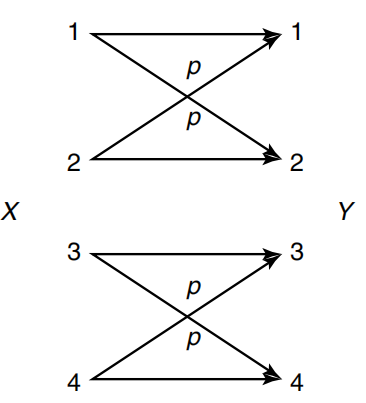
\includegraphics[width=0.3\textwidth]{../figures/7.34_a.png}
	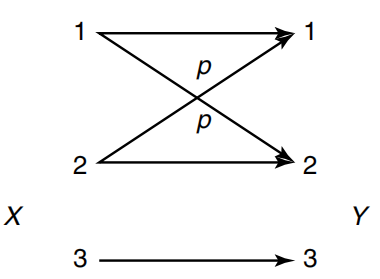
\includegraphics[width=0.3\textwidth]{../figures/7.34_b.png}
	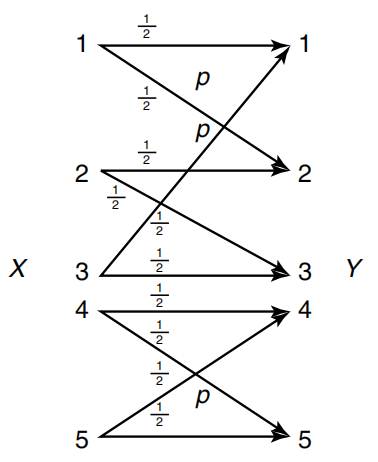
\includegraphics[width=0.3\textwidth]{../figures/7.34_c.png}
\end{figure}

(d) Ternary channel:
$$
p(y|x)=\left(\begin{array}{lll}
\frac{2}{3} & \frac{1}{3} & 0 \\
0 & \frac{1}{3} & \frac{2}{3}
\end{array}\right)
$$

\textcolor{blue}{Solution}

Since for (a), (b), (c): the channels are all combined with two parallel channels, so we can introduce two Lemmas.


Lemma1: If the channel is combined with two parallel channels with probability $\pi$ to the first channel, and $1-\pi$ to the second channel, which is as followed.
\begin{figure}[htbp]
    \centering
	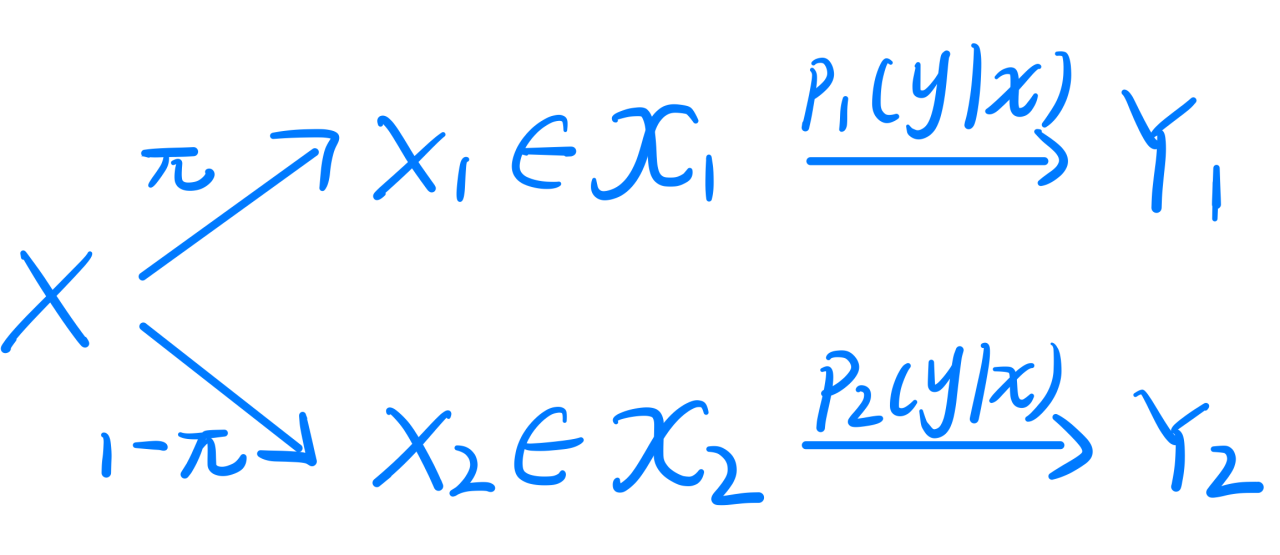
\includegraphics[width=0.3\textwidth]{../figures/parallel.png}
\end{figure}

Suppose the channel capacity of the total channel is $C$, and the capacity of the two channels are $C_1$ and $C_2$ respectively. Then we have
$$2^C=2^{C_1}+2^{C_2}$$
Proof: \\
Let $\Theta(X)$ be the auxiliary variable, indicating that $X$ is send to the $\Theta(X)$'s channel. Then we have
\begin{align*}
\Theta(X) &= \begin{cases}
1 & , X\in \mathcal{X}_1 \\
2 & , X\in \mathcal{X}_2 \\
\end{cases} \\
C_1 &= \max_{p_1(x)}I(X_;Y_1) \\
C_2 &= \max_{p_2(x)}I(X_;Y_2)
\end{align*}
And we also have that $p(\Theta=1)=p(X\in\mathcal{X}_1)=\pi, p(\Theta=2)=p(X\in\mathcal{X}_2)=1-\pi$.
And since when given $Y$ or given $X$, we could know $\Theta$, so we have $I(X;\Theta|Y)=H(\Theta|Y)-H(\Theta|X,Y)=0$.
i.e.
\begin{align*}
I(X;Y,\Theta) &= I(X;\Theta) + I(X;Y|\Theta) \\
&= I(X;Y) + I(X;\Theta|Y) = I(X;Y)
\end{align*}
Then we have
\begin{align*}
I(X;Y) &= I(X;\Theta) + I(X;Y|\Theta) \\
&= H(\Theta) - H(\Theta|X) + I(X;Y|\Theta) \\
&= H(\Theta) + I(X;Y|\Theta) \text{\qquad\qquad\quad ($\Theta$ is deterministic when $X$ is given)} \\
&= H\left(\pi,1-\pi\right) + I(X;Y|\Theta)
\end{align*}
As for $I(X;Y|\Theta)$, we have
\begin{align*}
I(X;Y|\Theta) &= H(X|\Theta) - H(X|Y,\Theta) \\
&= \sum_{\theta}p(\Theta=\theta)H(X|\Theta=\theta) - \sum_{\theta}p(\Theta=\theta)H(X|Y,\Theta=\theta) \\
&= \sum_{\theta}p(\Theta=\theta)\left[H(X|\Theta=\theta) - H(X|Y,\Theta=\theta)\right] \\
&= \sum_{\theta}p(\Theta=\theta)I(X;Y|\Theta=\theta) \\
&= \pi I(X_1;Y_1) + (1-\pi)I(X_2;Y_2) \\
&\leq \pi C_1 + (1-\pi)C_2 \text{\qquad\qquad ($C_1$ and $C_2$ are the capacity of the two channels)}
\end{align*}
So we have
$$I(X;Y) \leq H(\pi,1-\pi) \pi C_1 + (1-\pi)C_2 = -\pi\log \pi - (1-\pi)\log(1-\pi) + \pi C_1 + (1-\pi)C_2 \triangleq f(\pi)$$
Since we want to maximize $f(\pi)$, so it is obviously that $\pi=0$ or $\pi=1$ is not the optimal solution. And from the property of capcity, we have $C_1,C_2\geq 0$, so we have
\begin{align*}
f'(\pi) &= \log(1-\pi)-\log\pi+C_1-C_2 \\
f''(\pi) &= -\log_e2\left(\dfrac{1}{1-\pi}+\dfrac{1}{\pi}\right) < 0
\end{align*}
So $f(\pi)$ is a concave function, so the optimal solution is
$$f'(\pi^*)=0\Rightarrow \pi^*=\dfrac{2^{C_1}}{2^{C_1}+2^{C_2}}$$
So we have
\begin{align*}
C &= \max_{p(x)}I(X;Y) = \max_{\pi} f(\pi) = f(\pi^*) \\
&= \log \left(2^{C_1}+2^C_2\right)
\end{align*}
So we have proved that $2^C=2^{C_1}+2^{C_2}$. \qed

Lemma2: For a BSC. The probability of error is $p$, then the capacity is $1-H(p,1-p)$.
\begin{figure}[htbp]
    \centering
	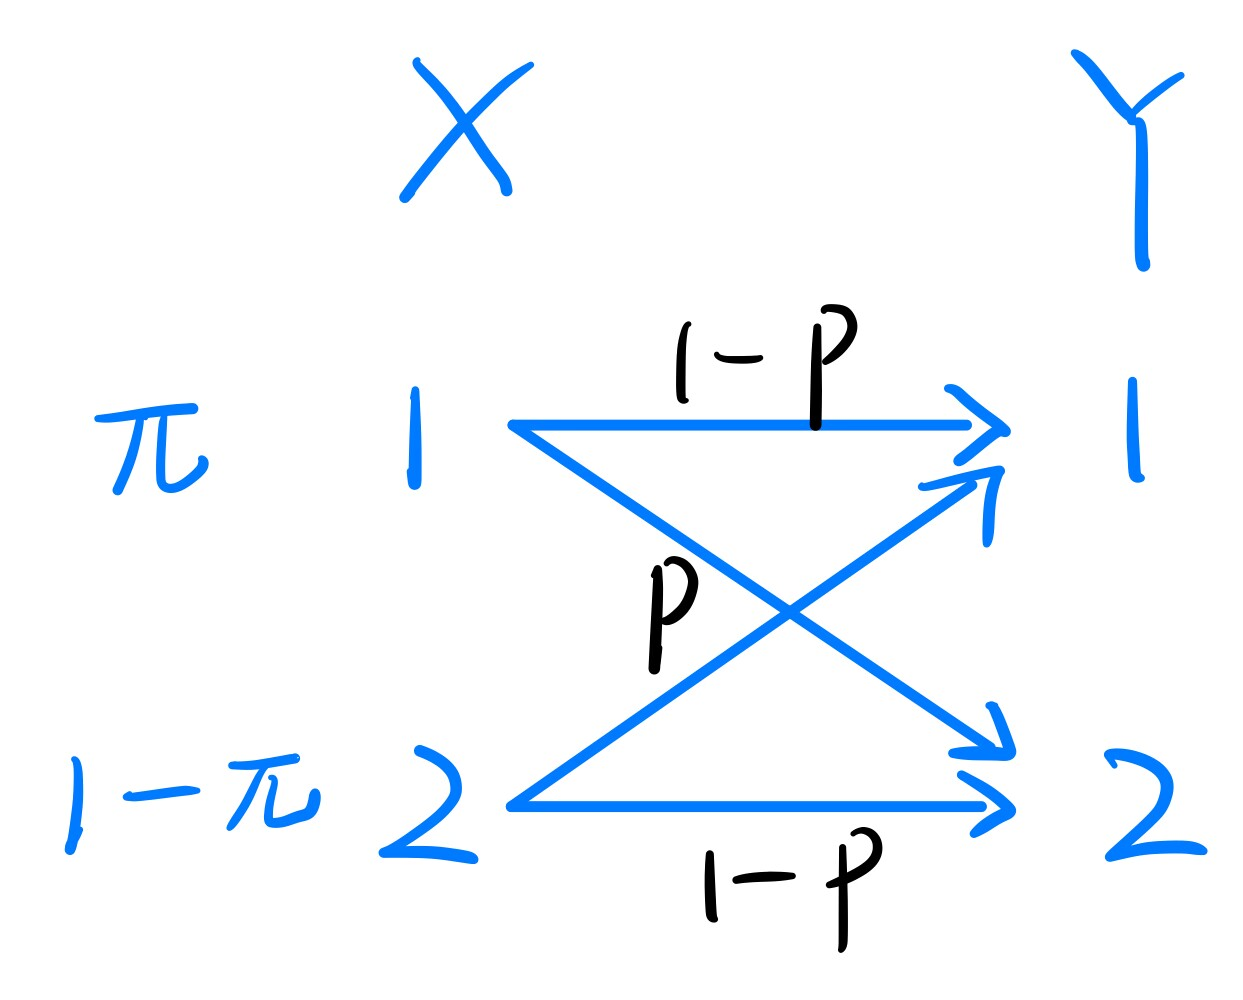
\includegraphics[width=0.3\textwidth]{../figures/BSC.png}
\end{figure}
\begin{align*}
I(X;Y) &= H(Y) - H(Y|X) \\
&= H(Y)-\sum_{x}p(x)H(Y|X=x) \\
&= H(Y) - H(p,1-p) \\
&\leq 1 - H(p,1-p)
\end{align*}
And we have when $P(X=1)=P(X=2)=\dfrac{1}{2}$, then $P(Y=0)=\sum\limits_xP(X=x)P(Y=1|X=x)=\dfrac{1}{2}$, and so does $P(Y=1)$.

So the inequality takes the equality, so we have when $p(x)=\left(\dfrac{1}{2},\dfrac{1}{2}\right)$
$$C=\max_{p(x)}I(X;Y)=1-H(p,1-p)$$
So with the two Lemmas, we could solve the problem easier. \\

(a) The two channels are paralleled BSC, so we have $C_1=C_2=1-H(p,1-p)$, so we have
$$C=\log\left(2^{1-H(p,1-p)}+2^{1-H(p,1-p)}\right)=2-H(p,1-p)$$

Where $\pi^*=\dfrac{2^{C_1}}{2^{C_1}+2^{C_2}}=\dfrac{1}{2}$.

When $p(x)=\left(\dfrac{1}{4},\dfrac{1}{4},\dfrac{1}{4},\dfrac{1}{4}\right)$, $I(X;Y)$ could take the maximum value.

(b) The first channel is a BSC, so $C_1=1-H(p,1-p)$. And for the second channel, $Y_2=X_2=3$, so
$$I(X_2;Y_2)=H(X_2)-H(X_2|Y_2)=H(X_2)=0$$
i.e. $C_2=0$. So we have
$$C=\log\left(2^{1-H(p,1-p)}+2^0\right)=\log\left(2^{1-H(p,1-p)}+1\right)$$

Where $\pi^*=\dfrac{2^{C_1}}{2^{C_1}+2^{C_2}}=\dfrac{2}{2+2^{H\left(p,1-p\right)}}$.

When $p(x)=\left(\dfrac{1}{2+2^{H\left(p,1-p\right)}},\dfrac{1}{2+2^{H\left(p,1-p\right)}},\dfrac{2^{H\left(p,1-p\right)}}{2+2^{H\left(p,1-p\right)}}\right)$, $I(X;Y)$ could take the maximum value. \\\\


(c) The second channel is a BSC, and $p=\dfrac{1}{2}$, so $C_2=1-H(p,1-p)=0$.

And for the first channel:
\begin{align*}
I(X;Y) &= H(Y) - H(Y|X) \\
&= H(Y) - \sum_{x}p(x)H(Y|X=x) \\
&= H(Y) - \sum_{x}p(x)H\left(\dfrac{1}{2},\dfrac{1}{2}\right) \\
&= H(Y) - 1 \\
&\leq \log 3 - 1
\end{align*}
When $p(X=1)=p(X=2)=p(X=3)=\dfrac{1}{3}$, we have
$$P(Y=1)=\sum_xP(X=x)P(Y=1|X=x)=\dfrac{1}{3}$$
Similarly, $P(Y=2)=P(Y=3)=\dfrac{1}{3}$. So the inequality takes the equality, so we have $C_1=\log 3 - 1$. \\
So we have
$$C=\log\left(2^0+2^{\log 3-1}\right)=\log 5 - 1$$

Where $\pi^*=\dfrac{2^{C_1}}{2^{C_1}+2^{C_2}}=\dfrac{3}{5}$ bit per transmission.

When $p(x)=\left(\dfrac{1}{5},\dfrac{1}{5},\dfrac{1}{5},\dfrac{1}{5},\dfrac{1}{5}\right)$, $I(X;Y)$ could take the maximum value.

(d)
\begin{align*}
I(X;Y) &= H(Y) - H(Y|X) \\
&= H(Y) - \sum_{x}p(x)H(Y|X=x) \\
&= H(Y) - H\left(\dfrac{1}{3},\dfrac{2}{3}\right) \\
&\leq \log 3 - H\left(\dfrac{1}{3},\dfrac{2}{3}\right)
\end{align*}
When $p(X=1)=p(X=2)=p(X=3)=\dfrac{1}{3}$, we have
$$P(Y=1)=\sum_xP(X=x)P(Y=1|X=x)=\dfrac{1}{3}$$
Similarly, $P(Y=2)=P(Y=3)=\dfrac{1}{3}$. So the inequality takes the equality. \\
So we have $C=\log 3 - H\left(\dfrac{1}{3},\dfrac{2}{3}\right)$. \\
And we have
$$H\left(\dfrac{1}{3},\dfrac{2}{3}\right) = -\dfrac{1}{3}\log\dfrac{1}{3}-\dfrac{2}{3}\log\dfrac{2}{3} = \log 3 - \dfrac{2}{3}$$

So above all, we have $C=\dfrac{2}{3}$ bit per transmission.

\newpage